\clearpage
%%=========================================
\section{MCT Film Grown by LPE on Substrate A}\label{sec:subAc}

A film of \acl{mct} was grown on substrate A by \ac{lpe}. Nomarski optical microscopy images reveal that the surface of the \ac{mct} film has wavy structures with a large number of circular features, as seen in Fig.~\ref{fig:subAc_om}. Two different kinds of circular features were observed: large circular defects with diameter of \SIrange{25}{40}{\micro\metre}, as seen in Fig.~\ref{fig:subAc_om_40um}, and donut-shaped defects \SIrange{10}{14}{\micro\metre} wide, as seen in Fig.~\ref{fig:subAc_om_10um}.

\begin{figure}[htbp]
    \centering
    \mySubfigure{0.49\textwidth}{LPE453_nomarski_grid_16_20x.jpg}[fig:subAc_om_centre][angle=180]
    \hfill
    \mySubfigure{0.49\textwidth}{LPE453_nomarski_grid_18_20x.jpg}[fig:subAc_om_edge][angle=180]
    \caption[Nomarski phase contrast microscopy images of \ac{mct} film grown by \ac{lpe} on substrate A.]{Nomarski phase contrast microscopy images of \ac{mct} film grown by \ac{lpe} on (111)B-oriented substrate A: \subref{fig:subAc_om_centre} Near the centre; and \subref{fig:subAc_om_edge} near the right edge.}
    \label{fig:subAc_om}
\end{figure}

\begin{figure}[htbp]
    \centering
    \mySubfigure{0.49\textwidth}{LPE453_om_5x_40um.png}[fig:subAc_om_40um][angle=180]
    \hfill
    \mySubfigure{0.49\textwidth}{LPE453_om_10um.png}[fig:subAc_om_10um][angle=180]
    \caption[Bright field optical microscopy images of defects seen on \ac{mct} film grown by \ac{lpe} on substrate A.]{Bright field optical microscopy images of: \subref{fig:subAc_om_40um} \SI{40}{\micro\metre} wide defect; and \subref{fig:subAc_om_10um} donut-shaped defects \SI{10}{\micro\metre} wide seen on \ac{mct} film grown by \ac{lpe} on (111)B-oriented substrate A.}
    \label{fig:subAc_om_40umand10um}
\end{figure}

The large defects are infrequent with respect to the donut-shaped defects. Only four large defects were observed in the lower right quadrant of the sample, which gives a density of \SI{\sim 2}{\centi\metre^{-2}}. The density of donut-shaped defects, on the other hand, was found to be between \SIrange{4e+3}{6e+4}{\centi\metre^{-2}}. The average density was \SI{2e+04}{\centi\metre^{-2}} with a standard deviation of \SI{1e+04}{\centi\metre^{-2}}. A graphical representation of the density at different locations on the film can be seen in Fig.~\ref{fig:LPE453_densityData}. \todo{Correlate with polishing grit density.}

\begin{figure}[htbp]
    \centering
    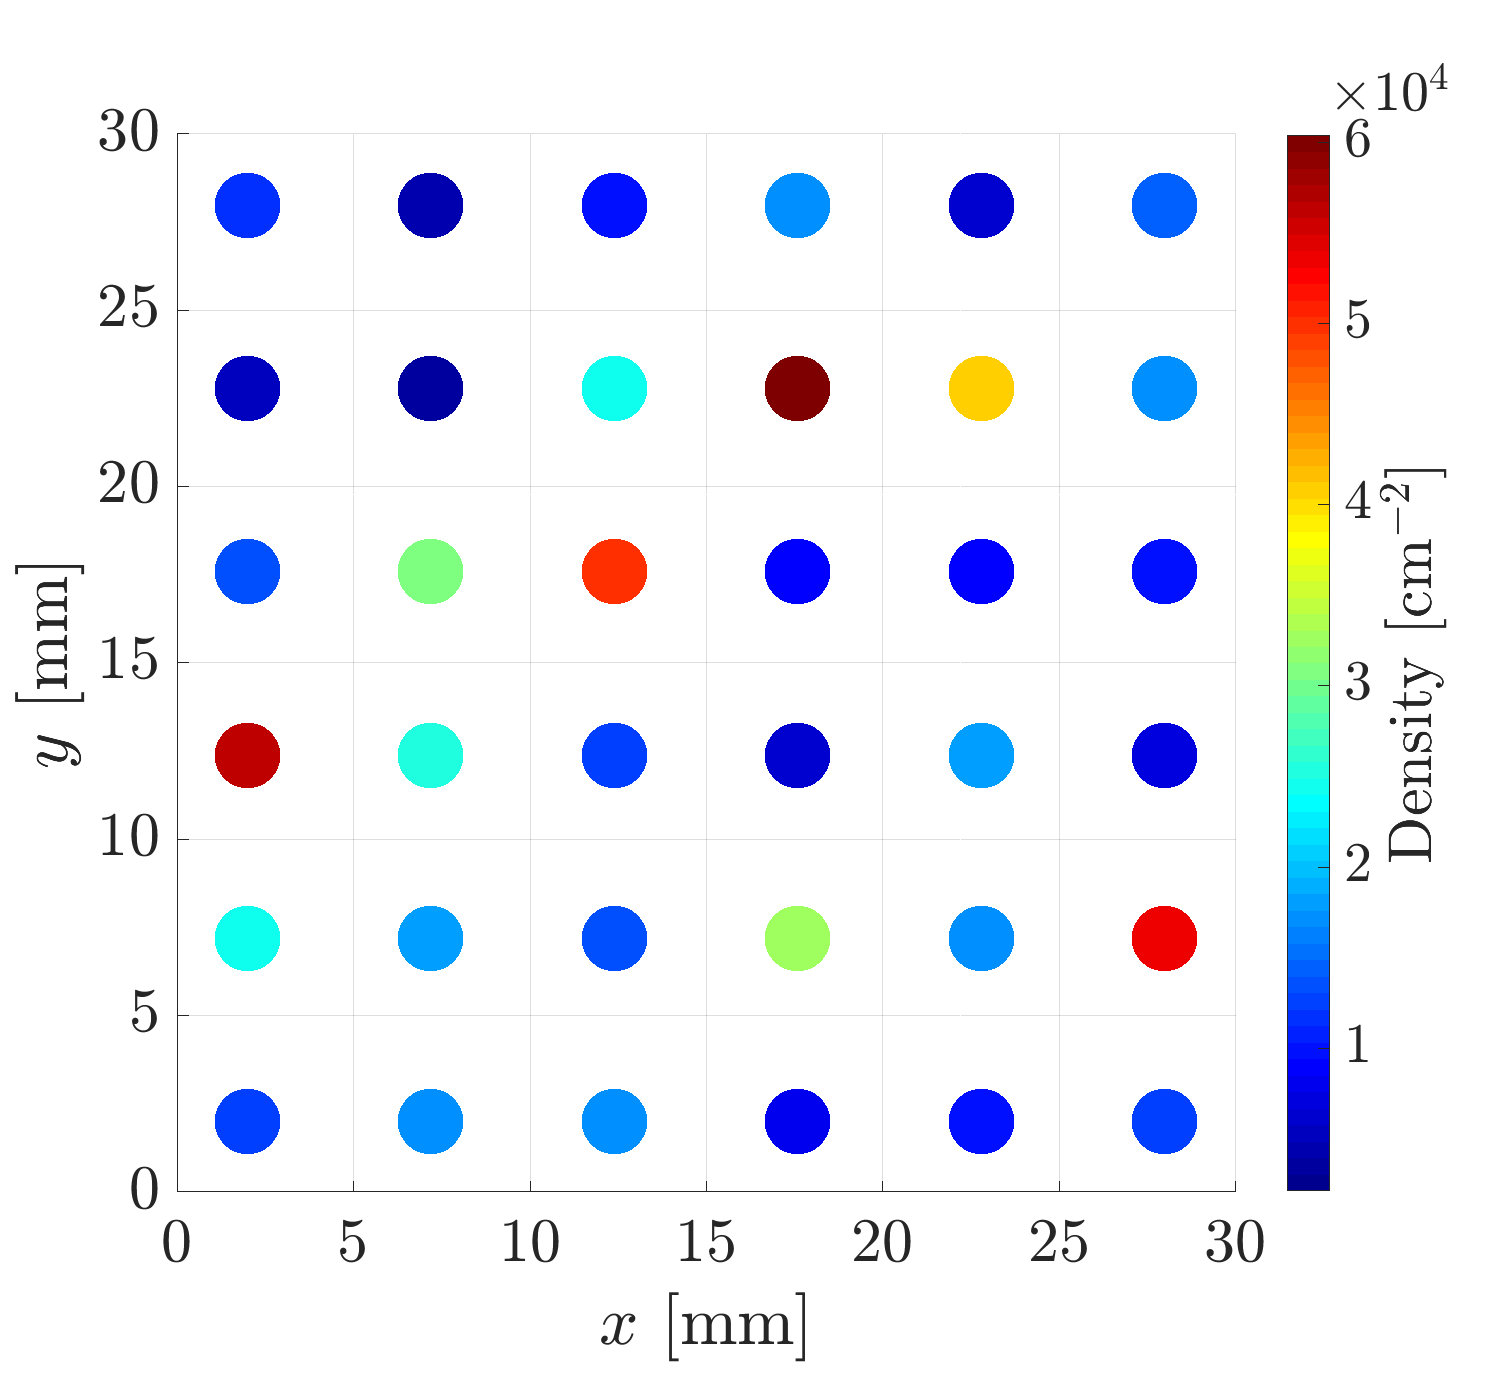
\includegraphics[width=0.5\linewidth]{LPE453_densityData.png}
    \caption[Map of the density of donut-shaped structures on the \ac{mct} film grown on substrate A.]{A map of the density of donut-shaped structures at 36 different locations on the $\SI{30}{\milli\metre}\times\SI{30}{\milli\metre}$ \ac{mct} film grown on substrate A. The density was observed to vary between \SIrange{4e+3}{6e+4}{\centi\metre^{-2}} with an average defect density of \SI{2e+04}{\centi\metre^{-2}}.}
    \label{fig:LPE453_densityData}
\end{figure}

%The circular shape of the large defects and the donut-shaped defects indicate that they are formed while the material were liquid during \ac{lpe}

%%=========================================
%\subsection{Particles and Surface Features}
%Seven different types of particles and surface features were observed on the surface of substrate B, see Fig.~\ref{fig:subBa_sem_w_eds}. They will be described and identified in the following.

%The presence of depressions or voids, which may, or may not, retain droplets of solution, can be interpretated according to the results published by Bauser [9, E. Bauser, AppI. Phys. 15 (1978) 243]. The presence on the substrate of defects like oxide, microprecipitates, graphite particles prevents the wetting of the substrate by the liquid phase and can induce voids or depressions.Fig. 6 illustrates this mechanism.


%%=========================================
\subsection{Composition and Thickness}

\todo{FTIR: correlate with polishing grit or donut density.}

%%=========================================
\subsection{Impurity Analysis}

\Ac{eds} was used to get a quantitative analysis of the chemical composition of the \ac{mct} film grown by \ac{lpe} on substrate A. The results can be seen in Table~\ref{tab:subAc_eds_analysis}. The following elements were identified: \ce{Te}, \ce{Hg}, \ce{Cd}, \ce{C}, \ce{O}, and \ce{Al}. The relative concentrations of \ce{Cd}, \ce{Zn}, and \ce{Te} were \ce{Hg_{0.71}Cd_{0.29}Te}, \ce{Hg_{0.77}Cd_{0.23}Te}, and \ce{Hg_{0.76}Cd_{0.24}Te} for the centre, edge, and corner respectively. 


\begin{table}[htbp]
    \centering
    \caption[\Ac{eds} impurity analysis of \ac{mct} film grown by \ac{lpe} on substrate A.]{Results of the \ac{eds} impurity analysis at three different locations on the $30\times30$ \SI{}{\milli\metre^2} \ac{mct} film grown by \ac{lpe} on (111)B-oriented substrate A (atomic concentration \%). The X-ray signal is acquired from $\SI{1270}{\micro\metre}\times\SI{890}{\micro\metre}$ areas near the centre, upper edge, and upper left corner.}\label{tab:subAc_eds_analysis}
   \begin{tabu} to 1.0\textwidth { X[1.85, r] X[1.125,c] X[1.125,c] X[1.125,c] X[1.125,c] X[1.125,c] X[1.125,c] }
        \hline
            & \textbf{\ce{Te}} (at.\%) & \textbf{\ce{Hg}} (at.\%) & \textbf{\ce{Cd}} (at.\%) & \textbf{\ce{C} } (at.\%) & \textbf{\ce{O}} (at.\%) & \textbf{\ce{Al}} (at.\%) \\
        \hline
        Near centre & \SI{43,96}{} & \SI{30,82}{} & \SI{12,39}{} & \SI{11,38}{} & \SI{1,28}{} & \SI{0,17}{} \\
        Near edge & \SI{43,87}{} & \SI{33,27}{} & \SI{9,8}{} & \SI{11,7}{} & \SI{1,13}{} & \SI{0,23}{} \\
        Near corner & \SI{43,58}{} & \SI{32,74}{} & \SI{10,24}{} & \SI{11,98	}{} & \SI{1,18}{} & \SI{0,27}{}  \\
        \hline
    \end{tabu}
\end{table}
%%=========================================